\documentclass[
    table,
    12pt,
    oneside,
    a4paper,
    italian
]{book}

\input{config/packages}
\input{config/thesis_config}

\date{}

\hypersetup{pdfstartview=}
\begin{document}
    \frontmatter
    \input{preface/1_title_page}
    \increasepagenumbering
    \input{preface/2_copyright}
    %\cleardoublepage
\phantomsection
\pdfbookmark{Ringraziamenti}{Ringraziamenti}

\begin{flushright}{
    \slshape
    ``Se fai solo quello che sai fare, non sarai mai più di quello che sei ora.''} \\
    \medskip
\end{flushright}

\begingroup
\let\clearpage\relax
\let\cleardoublepage\relax
\let\cleardoublepage\relax

\chapter*{Ringraziamenti}

\vspace{0.35cm}

\noindent Prima di tutto, desidero ringraziare profondamente la mia famiglia: mia mamma Katia, mio papà Andrea e, \textit{soprattutto}, mio fratello Gabriele, per l'immenso e costante supporto che mi hanno sempre dato durante tutto il mio percorso di laurea.

\vspace{0.35cm}

\noindent Vorrei poi porgere i miei ringraziamenti ai ``Poti'' e alle ``Pote'', che hanno reso indimenticabili questi tre anni di università, condividendo con me lo studio, l'ansia degli esami e innumerevoli risate.

\vspace{0.35cm}

\noindent Un pensiero speciale va a tutti i miei amici, che mi sono stati a fianco e mi hanno incoraggiato durante la stesura di questa tesi.

\vspace{0.35cm}

\noindent Infine, desidero ringraziare il mio relatore, il Professor Tullio Vardanega, per la disponibilità, il rigore e il prezioso aiuto che mi ha fornito durante la stesura di questo elaborato.

\vspace{0.75cm}

\noindent{\myLocation, \myTime}
\hfill \textit{\myName}

\endgroup
    \cleardoublepage
\phantomsection
\pdfbookmark{Compendio}{Compendio}
\begingroup
\let\clearpage\relax
\let\cleardoublepage\relax
\chapter*{Sommario}
Il presente documento descrive il lavoro svolto durante il periodo di \textit{stage}, dal 5 maggio 2026 al 1 luglio 2026, presso l'azienda Ergon Informatica S.r.l..

\noindent
Il percorso di tirocinio è stato monitorato dal Prof. Tullio Vardanega e dal tutor aziendale Thomas Garbui e ha avuto come obiettivo principale la realizzazione di una \textit{web application} per la gestione logistica delle prenotazioni di banchine di scarico per mezzi pesanti, mediante lo sviluppo con \textit{React} e \textit{C\#}.

\noindent
Il documento è suddiviso in \textbf{4 capitoli}:
\begin{itemize}
    \item \textbf{Capitolo 1: Ergon Informatica S.r.l. - Ambito organizzativo e metodologie di lavoro}. Viene descritta la struttura organizzativa dell'azienda, le metodologie di lavoro adottate e le tecnologie utilizzate nel contesto del tirocinio.
    \item \textbf{Capitolo 2: Strategia aziendale e obiettivi del percorso di tirocinio}. Viene analizzato il ruolo del tirocinio all'interno della filosofia di innovazione, confrontando le motivazioni alla base della proposta progettuale e la rispondenza del progetto alle esigenze di mercato.
    \item \textbf{Capitolo 3: Kargo - Progetto di tirocinio}. Viene presentato il progetto di tirocinio, descrivendo il ciclo di vita del \textit{software}, le tecnologie utilizzate, le decisioni progettuali e le funzionalità implementate nell'applicativo.
    \item \textbf{Capitolo 4: Valutazione retrospettiva}. Viene effettuata un'analisi critica dei risultati ottenuti dallo \textit{stagiaire}, comparando le aspettative iniziali con i risultati finali, e misurando l'impatto del tirocinio sullo sviluppo delle competenze professionali e personali.
\end{itemize}
\newpage
\chapter*{Convenzioni Tipografiche}
Al fine di rendere più chiara la lettura del documento, sono state adottate le seguenti convenzioni tipografiche:
\begin{itemize}
    \item Il \textit{corsivo} è utilizzato per evidenziare termini in lingua straniera, titoli di opere o documenti, e per enfatizzare concetti o parole chiave.
    \item Le immagini e le figure sono numerate progressivamente e accompagnate da una didascalia descrittiva che ne chiarisce il contesto.
    \item I codici sorgente sono presentati in un font monospazio, con numerazione delle righe e indentazione coerente per facilitarne la consultazione.
    \item I termini contrassegnati dal simbolo $^{G}$ in apice sono definiti all'interno del glossario, a cui si rimanda per un approfondimento terminologico.
\end{itemize}
\endgroup
\vfill

    \input{preface/5_table_of_contents}
    \blankpage

    \mainmatter
    \chapter{Ergon Informatica S.r.l}
\label{chap:introduzione}


\textit{Il presente capitolo delinea il contesto operativo all'interno del quale si è svolta l'attività di tirocinio. Attraverso un'analisi della struttura aziendale e delle metodologie di sviluppo adottate, si intende definire il quadro di riferimento per comprendere le successive decisioni progettuali, il contesto in cui opera e l'importanza verso l'innovazione e il miglioramento continuo. Le informazioni qui riportate sono state raccolte mediante l'osservazione attiva dei flussi di lavoro, l'analisi della documentazione tecnica interna e il confronto con le figure di riferimento aziendale.}

\section{Profilo aziendale}
In questa sezione viene descritta l'identità di Ergon Informatica S.r.l., ripercorrendone brevemente la storia e il posizionamento strategico nel panorama IT. Sono analizzati i principali domini applicativi di riferimento e la tipologia di clientela servita, fornendo una visione d'insieme atta a contestualizzare la rilevanza del tirocinio.


\section{Metodologie di sviluppo e processi operativi}
Viene analizzato il ciclo di vita del \textit{software} adottato in azienda, mettendo in luce le pratiche metodologiche che guidano il team di sviluppo dal recepimento dei requisiti fino al rilascio. Particolare attenzione è rivolta agli strumenti tecnologici utilizzati e alle procedure di manutenzione, supportate da schemi e flussi che testimoniano l'approccio rigoroso dell'azienda.

\section{Innovazione tecnologica e cultura aziendale}
La seguente sezione esplora la propensione di Ergon verso l'innovazione ed il miglioramento continuo. Attraverso l'analisi delle scelte tecnologiche e della cultura aziendale, si evidenzia come tali elementi abbiano influito direttamente sul progetto di tirocinio, ponendo le basi per l'analisi dei capitoli successivi.

\newpage
    \chapter{Lo \textit{stage} come innovazione}
\label{chap:strategia}

\textit{Nel presente capitolo approfondisco le motivazioni strategiche alla base della proposta di tirocinio, inserendola nel più ampio quadro della visione aziendale di Ergon Informatica. Mediante l'analisi degli obiettivi formativi e dei vincoli progettuali, analizzo e illustro come il tirocinio si inserisca nella strategia aziendale di innovazione e di miglioramento continuo dei processi, configurandosi sia come occasione di crescita per il candidato sia come strumento attraverso cui l'organizzazione esplora nuove soluzioni tecnologiche. Traggo le considerazioni riportate principalmente dalle interviste svolte con il tutor aziendale e dalle osservazioni raccolte durante il periodo di permanenza in azienda.}

\section{Il valore dello \textit{stage} in Ergon Informatica}
\label{sec:valore_stage}

Come discusso nella Sezione~\ref{subsec:ruolo_tirocini}, Ergon Informatica considera il tirocinio uno degli strumenti principali per l'esplorazione tecnologica. Per alimentare costantemente questo ecosistema di sperimentazione, l'organizzazione ha strutturato una solida rete di collaborazioni con le principali istituzioni formative del territorio, accogliendo annualmente oltre una decina di tirocinanti. 

\subsection{Collaborazioni con le istituzioni formative}
\label{subsec:collaborazioni_formative}

L'azienda seleziona candidati da provenienze volutamente eterogenee: esse spaziano dai percorsi accademici tradizionali, come l'Università degli Studi di Padova e l'Università Ca' Foscari di Venezia, fino a iter maggiormente professionalizzanti come i vari Istituti Tecnici Superiori (ITS) della regione. 

Questa diversificazione consente all'azienda di individuare con continuità nuovi talenti e, ancor più importante, le permette di importare approcci mentali e operativi differenti. Come illustro nella Tabella~\ref{tab:confronto_profili_tirocinio}, mentre i profili universitari tendono ad apportare un maggiore rigore ingegneristico e metodologico, i profili tecnici introducono spesso una spiccata propensione per l'operatività immediata. 

\begin{table}[H]
    \centering
    \begin{tabular}{p{0.35\textwidth} p{0.55\textwidth}}
        \hline
        \textbf{Profilo del Tirocinante} & \textbf{Contributo Metodologico e Operativo} \\
        \hline
        Percorsi Accademici Universitari & Rigore ingegneristico, approfondimento teorico e approccio strutturato \\
        Istituti Tecnici Superiori & Immediatezza esecutiva, pragmatismo operativo e orientamento pratico \\
        \hline
    \end{tabular}
    \caption{Diversificazione degli approcci metodologici apportati dai tirocinanti.}
    \vspace{0.1cm}
    {\footnotesize Elaborazione originale dell'autore\par}
    \label{tab:confronto_profili_tirocinio}
\end{table}

L'inserimento di queste risorse consente inoltre all'organizzazione di osservare indirettamente l'evoluzione del panorama tecnologico e formativo esterno. Il confronto con studenti provenienti da percorsi differenti permette ai responsabili di raccogliere indicazioni sulle tecnologie maggiormente diffuse nei percorsi di studio, sugli strumenti emergenti e sugli approcci metodologici più recenti. In tale prospettiva, i tirocinanti diventano il collegamento tra il contesto accademico e quello industriale.

\subsection{Integrazione del tirocinante nel contesto aziendale}
\label{subsec:integrazione_tirocinante}

Sulla base delle informazioni raccolte, ho potuto comprendere come Ergon progetti generalmente le attività di tirocinio evitando mansioni esclusivamente esecutive o a basso valore formativo. I responsabili concepiscono le iniziative per coniugare le esigenze concrete dell'organizzazione con gli interessi e il percorso del candidato, con l'obiettivo di generare un coinvolgimento attivo e favorire la validazione di soluzioni con potenziale impatto reale. 

Questo approccio favorisce uno scambio di competenze all'interno dell'azienda: i tirocinanti beneficiano della profonda conoscenza del dominio applicativo e delle logiche commerciali trasferite dai colleghi esperti, mentre le figure \textit{senior} entrano in contatto con tecnologie emergenti e paradigmi moderni portati dai più giovani. In questo scenario, il tirocinante non assume il ruolo di semplice esecutore, ma contribuisce attivamente allo studio di strumenti e approcci alternativi, offrendo all'organizzazione l'opportunità di osservare nuove modalità operative e valutarne l'eventuale adozione futura.

\section{Ciclo di vita del tirocinio}
\label{sec:ciclo_vita_tirocinio}
Affinché l'apporto innovativo dei tirocinanti si traduca in un \textit{asset} tangibile e non in una dispersione di energie, Ergon ha istituzionalizzato un modello operativo rigoroso: l'azienda inserisce ogni progetto formativo in un ciclo di vita continuo, la cui architettura prevede un chiaro "prima" e un altrettanto definito "dopo" rispetto all'orizzonte temporale dello studente in sede.

\subsection{La genesi del progetto}
\label{subsec:genesi_necessita}

Il ciclo di vita di un progetto di \textit{stage} inizia molto prima dell'arrivo del candidato. La direzione definisce le iniziative partendo da problematiche operative concrete, che scaturiscono da due fonti primarie: 
\begin{itemize}
    \item \textbf{Impulsi di mercato:} specifiche richieste della clientela per funzionalità moderne che il gestionale storico non è in grado di erogare agilmente, come ad esempio cruscotti \textit{web} interattivi, interfacce \textit{mobile} per gli operatori logistici o portali di comunicazione \gls{b2b} --- ovvero sistemi concepiti per l'interazione commerciale diretta tra aziende, senza l'intermediazione del consumatore finale.
    \item \textbf{Esigenze infrastrutturali interne:} colli di bottiglia architettonici che la dirigenza tecnica rileva e che richiedono un'indagine preliminare su strumenti più efficienti --- quali moderni \gls{orm}, una tecnica di programmazione che mappa le tabelle di una base di dati relazionale su oggetti del codice sorgente per semplificarne la persistenza, o architetture \gls{restful}, uno stile architetturale per lo sviluppo di servizi \textit{web} standardizzati e disaccoppiati basati sul protocollo HTTP --- prima di una loro adozione definitiva.
\end{itemize}

Quando emerge una di queste esigenze, il \textit{team} tecnico ne delimita il perimetro funzionale e individua uno \textit{stack} tecnologico coerente con gli obiettivi esplorativi del progetto. Il gruppo di lavoro traduce così il problema operativo in un'attività di tirocinio delimitata e verificabile, destinata a produrre sia un risultato concreto sia elementi utili alla valutazione di possibili evoluzioni tecnologiche.

\subsection{Il processo di validazione tecnica}
\label{subsec:validazione_tecnica}

Secondo il modello organizzativo illustrato dal tutor aziendale, la conclusione formale del tirocinio, coincidente con il completamento del monte ore previsto, rappresenta generalmente per l'azienda l'inizio di una fase di consolidamento dei risultati ottenuti. In questa fase, l'azienda persegue l'obiettivo di produrre un modulo sufficientemente autonomo da poter essere valutato in termini tecnici e organizzativi; anche nei casi in cui il livello di completezza non consenta un impiego immediato, la dirigenza conserva e considera normalmente il lavoro svolto come base di riferimento per sviluppi successivi.

Al termine dello \textit{stage}, gli sviluppatori \textit{senior} sottopongono il codice sorgente, le scelte architetturali effettuate, la documentazione redatta e le pratiche di collaudo a una rigorosa procedura di \textit{code review}. I responsabili tecnici non si limitano a verificare il funzionamento dell'interfaccia, ma effettuano un \textit{audit} approfondito per valutare la manutenibilità del codice, la sicurezza delle \gls{api} --- le interfacce di programmazione che permettono ad applicativi diversi di comunicare e scambiare dati in modo standardizzato --- e la reale scalabilità delle tecnologie proposte dal tirocinante.

\subsection{Integrazione e sviluppo iterativo}
\label{subsec:integrazione_sviluppo}

A seguito del processo di validazione, il codice generato confluisce nel patrimonio informativo aziendale seguendo una di due possibili traiettorie di integrazione, a seconda della maturità del prodotto e della complessità del dominio affrontato:

\begin{enumerate}
    \item \textbf{Messa in produzione diretta:} Se l'applicativo soddisfa i rigidi requisiti di affidabilità aziendali e lo \textit{stack} tecnologico impiegato ha dimostrato la robustezza attesa, il \textit{software} entra in una fase di rifinitura interna. Gli sviluppatori \textit{senior} collegano il modulo sperimentale ai sistemi di persistenza di produzione e procedono con il rilascio progressivo ai clienti. In questo scenario, il tirocinio ha fornito all'azienda un prodotto commerciale "chiavi in mano".
    \item \textbf{Sviluppo iterativo e passaggio di consegne:} Qualora il progetto affronti un dominio applicativo troppo vasto per essere esaurito nel tempo a disposizione, o se la tecnologia investigata richiede ulteriori validazioni architetturali, il lavoro dello stagista assume il ruolo di \textit{baseline} (versione di riferimento). La dirigenza tecnica congela tale base di partenza e la riassegna successivamente come punto di inizio per un tirocinante futuro. Questo approccio a "staffetta" permette di aggredire problemi complessi suddividendoli in più cicli formativi, generando iterativamente valore incrementale.
\end{enumerate}

In entrambi gli scenari, il tirocinio contribuisce ad arricchire il patrimonio tecnico e organizzativo dell'azienda: da un lato attraverso la produzione di componenti o conoscenze riutilizzabili, dall'altro fornendo elementi utili per orientare le future decisioni di evoluzione tecnologica del sistema informativo. La Figura~\ref{fig:ciclo_tirocini_ergon} riassume visivamente l'intero ciclo di vita esplorativo, dalla raccolta delle necessità iniziali fino alla diramazione conclusiva tra produzione e sviluppo iterativo.

\begin{figure}[H]
    \centering
    \resizebox{\textwidth}{!}{
    \begin{tikzpicture}[
        node distance=1.5cm and 2cm,
        box/.style={rectangle, draw=black, thick, fill=blue!5, text width=4cm, align=center, minimum height=1.2cm, font=\small},
        decision/.style={diamond, aspect=2, draw=black, thick, fill=orange!10, text width=2.5cm, align=center, font=\footnotesize, inner sep=0pt},
        arrow/.style={thick, ->, >=stealth}
    ]
        % Nodi
        \node[box] (input) {\textbf{Genesi}\\Impulsi mercato o\\esigenze interne};
        \node[box, below=1cm of input] (sviluppo) {\textbf{Fase di Tirocinio}\\Sviluppo PoC / MVP};
        \node[box, below=1cm of sviluppo] (review) {\textbf{Validazione}\\\textit{Code Review} e \textit{Audit}};
        \node[decision, below=1cm of review] (bivio) {Maturità\\Progetto};
        \node[box, left=1cm of bivio] (prod) {\textbf{Messa in Produzione}\\Integrazione e rilascio};
        \node[box, right=1cm of bivio] (iter) {\textbf{Sviluppo Iterativo}\\\textit{Baseline} per futuri \textit{stage}};

        % Frecce
        \draw[arrow] (input) -- (sviluppo);
        \draw[arrow] (sviluppo) -- (review);
        \draw[arrow] (review) -- (bivio);
        \draw[arrow] (bivio) -- node[above=0.15cm, font=\footnotesize] {} (prod);
        \draw[arrow] (bivio) -- node[above=0.15cm, font=\footnotesize] {} (iter);
        
        % Freccia di ritorno per sviluppo iterativo
        \draw[arrow, dashed] (iter.north) |- node[above right=0.15cm, font=\footnotesize] {Nuovo ciclo} (sviluppo.east);
    \end{tikzpicture}
    }
    \caption{Rappresentazione schematica del ciclo di vita dei progetti in Ergon.}
    \vspace{0.1cm}
    {\footnotesize Elaborazione originale dell'autore\par}
    \label{fig:ciclo_tirocini_ergon}
\end{figure}

\section{Il dominio applicativo del progetto Kargo}
\label{sec:dominio_logistico}

In aderenza alle logiche di assegnazione precedentemente descritte, il mio progetto di tirocinio --- denominato "Kargo" --- trae origine da una specifica esigenza di mercato. Un cliente di Ergon Informatica, operante nel settore della distribuzione di bevande, ha manifestato la necessità di risolvere una forte criticità legata alla logistica \textit{inbound}: la congestione delle banchine di scarico. 

Nella gestione quotidiana dei magazzini, l'arrivo non programmato dei vettori e la simultaneità delle consegne generano inefficienze a catena. I magazzinieri subiscono picchi di lavoro imprevedibili, con conseguenti ritardi nello stoccaggio, mentre i corrieri sono costretti a lunghi periodi di attesa nei piazzali prima di poter effettuare le operazioni di scarico, con un inevitabile aggravio dei costi operativi.

L'azienda, incaricata di fornire una soluzione, aveva inizialmente pianificato uno sviluppo interno tradizionale. Tuttavia, riconoscendo in questa specifica problematica le dimensioni ideali per uno \textit{stage} e dopo aver valutato la necessità di esplorare nuove tecnologie \textit{web}, la dirigenza ha deciso di convertire la commessa in un progetto di tirocinio esplorativo.

\subsection{Obiettivi e vincoli del progetto Kargo}
\label{subsec:obiettivi_vincoli_kargo}

Attraverso un confronto diretto con il mio tutor aziendale, abbiamo definito congiuntamente il perimetro operativo del progetto Kargo, tracciando obiettivi funzionali chiari e quantificabili, e imponendo vincoli architetturali strategici.

\textbf{L'obiettivo funzionale aziendale} consisteva nello sviluppo di un'applicazione \textit{web} in grado di digitalizzare e automatizzare la prenotazione degli \textit{slot} temporali per lo scarico merci. L'applicativo doveva consentire ai corrieri di monitorare le disponibilità delle banchine in tempo reale, prenotare un appuntamento in modo sicuro e fornire all'amministrazione uno strumento di pianificazione ordinata. Per valutare oggettivamente il raggiungimento del risultato, Ergon ha fissato l'aspettativa di ricevere, entro le 300 ore previste dal tirocinio, un \gls{mvp} --- ovvero una versione iniziale del \textit{software} limitata alle funzionalità essenziali per completare un intero ciclo logistico (dalla registrazione del corriere alla conferma dello \textit{slot}) e raccogliere i riscontri dei committenti --- strutturalmente idoneo a essere rifinito e presentato al cliente.

\textbf{I vincoli tecnologici e architetturali} stabiliti da Ergon sono stati altrettanto rigorosi. L'azienda ha richiesto espressamente l'utilizzo del \textit{framework} React per lo sviluppo del livello di presentazione (\textit{frontend}), una tecnologia inedita rispetto agli standard interni. Inoltre, ha imposto un vincolo di stretta modularità architetturale: ho dovuto progettare il sistema per renderlo agilmente integrabile, in un secondo momento, con il gestionale \textit{legacy} proprietario descritto in Sezione~\ref{subsec:ecosistema_applicativo}. Questo requisito ha reso necessario un approccio disaccoppiato, basato sullo sviluppo di API in ambiente .NET per il livello logico. La Figura~\ref{fig:vincoli_architettura_kargo} illustra questa netta separazione strutturale, evidenziando il perimetro operativo assegnato al progetto Kargo e le relative modalità di comunicazione con il preesistente livello di persistenza.

\begin{figure}[H]
    \centering
    \resizebox{\textwidth}{!}{
    \begin{tikzpicture}[
        node distance=3cm,
        box/.style={rectangle, draw=black, thick, text width=4cm, align=center, minimum height=1.8cm, font=\small},
        arrow/.style={thick, <->, >=stealth}
    ]
        % Nodi con colori distintivi leggeri
        \node[box, fill=cyan!10] (frontend) {\textbf{Livello Presentazione}\\Applicazione Web\\(React)};
        \node[box, fill=green!10, right=2.5cm of frontend] (api) {\textbf{Livello Logico}\\Servizi RESTful\\(.NET C\#)};
        \node[box, fill=red!10, right=2.5cm of api] (legacy) {\textbf{Livello Persistenza}\\\textit{Database} Informix};

        % Frecce
        \draw[arrow] (frontend) -- node[above=0.15cm, font=\footnotesize] {Richieste HTTP} node[below=0.15cm, font=\footnotesize] {JSON} (api);
        \draw[arrow] (api) -- node[above=0.15cm, font=\footnotesize] {Integrazione} node[below=0.15cm, font=\footnotesize] {Legacy} (legacy);
        
        % Riquadro di raggruppamento ancorato automaticamente
        \draw[dashed, thick, draw=gray] 
            ([xshift=-0.5cm, yshift=0.9cm]frontend.north west) 
            rectangle 
            ([xshift=0.5cm, yshift=-0.5cm]api.south east);
            
        % Testo del perimetro
        \node[font=\footnotesize, text=gray, anchor=north west] 
            at ([xshift=-0.4cm, yshift=0.8cm]frontend.north west) 
            {Perimetro di sviluppo del progetto Kargo};

    \end{tikzpicture}
    }
    \caption{Vincoli di modularità architetturale imposti per il progetto Kargo.}
    \vspace{0.1cm}
    {\footnotesize Elaborazione originale dell'autore\par}
    \label{fig:vincoli_architettura_kargo}
\end{figure}

\section{Motivazioni e traguardi personali}
\label{sec:motivazioni_scelta}

Durante la fase di selezione delle proposte di \textit{stage}, la mia candidatura iniziale era in realtà orientata verso un differente progetto interno, relativo allo sviluppo di un sistema per il controllo degli accessi aziendali basato su tecnologia .NET MAUI. Tuttavia, a seguito di un colloquio orientativo con la direzione delle Risorse Umane, l'azienda mi ha proposto il progetto Kargo, illustrandone lo \textit{stack} tecnologico, le problematiche da risolvere e gli obiettivi. Ho quindi scelto di orientare il mio percorso formativo verso quest'ultima proposta per motivazioni di natura sia tecnologica sia metodologica.

In primo luogo, dal punto di vista tecnico, Kargo rappresentava l'unica iniziativa a proporre lo sviluppo di interfacce tramite React. Rispetto alle alternative basate su \textit{framework} maggiormente legati all'ecosistema \textit{desktop} o \textit{mobile} ibrido, l'opportunità di confrontarmi con lo sviluppo \textit{web full-stack} moderno ha costituito per me un incentivo professionale determinante. 

In secondo luogo, dal punto di vista metodologico, la natura esplorativa del progetto si allineava perfettamente con i miei obiettivi accademici. Durante il percorso universitario, ed in particolare nel corso di Ingegneria del Software, ho sviluppato un forte interesse per le tematiche relative al \gls{system_design} --- l'insieme delle metodologie di progettazione dell'architettura e dei componenti di sistemi informatici complessi --- e all'architettura del \textit{software}. Un progetto nato al di fuori dei rigidi binari della produzione standard mi offriva un maggiore margine di manovra: garantiva la libertà necessaria per progettare un sistema \textit{ex novo}, permettendomi di applicare con rigore i \textit{pattern} architetturali appresi e di analizzare criticamente le mie scelte ingegneristiche in un ambiente protetto.

A fronte di queste premesse, ho stabilito dei traguardi personali oggettivi, articolati nei seguenti punti:
\begin{itemize}
    \item \textbf{Padronanza tecnologica e metodologica:} raggiungere la piena autonomia operativa nello sviluppo di applicazioni basate su C\# e React, comprovata dalla consegna dell'MVP nei tempi stabiliti, e sviluppare parallelamente un metodo di studio efficiente per assimilare rapidamente nuovi linguaggi di programmazione.
    \item \textbf{Architettura e \textit{problem solving}:} progettare un'architettura \textit{software} applicando consapevolmente i principi di \textit{System Design}, che ottenga la validazione positiva del \textit{team} tecnico durante le procedure di \textit{code review}.
    \item \textbf{Gestione del ciclo di vita del \textit{software}:} condurre operativamente tutte le principali fasi di produzione, tracciando il passaggio dalla progettazione iniziale alla validazione finale.
\end{itemize}

Mi sono posto l'obiettivo di verificare quanto le conoscenze teoriche acquisite durante il corso di laurea fossero effettivamente applicabili in un contesto industriale, consolidandole attraverso lo svolgimento diretto delle attività progettuali. I traguardi definiti in questa sezione costituiranno quindi il riferimento metrico con cui, nel Capitolo~\ref{chap:conclusioni}, valuterò oggettivamente i risultati ottenuti al termine del tirocinio.
    \chapter{Sviluppare Kargo}
\label{chap:progettazione-codifica}

\textit{Il presente capitolo documenta le fasi operative del progetto Kargo, illustrando il metodo di lavoro adottato e il percorso di sviluppo che ha condotto alla realizzazione dell'applicativo. Attraverso l'analisi del ciclo di vita del software e delle principali sfide progettuali, descrivo il percorso che ha condotto dalla definizione dei requisiti iniziali alla realizzazione e validazione dell'applicativo.}

\section{Metodologia di lavoro e interazione}
\label{sec:metodologia_lavoro}

Per garantire il corretto avanzamento del progetto all'interno del limitato orizzonte temporale dello \textit{stage}, ho definito con il tutor aziendale un perimetro metodologico chiaro, stabilendo le regole di comunicazione e i criteri di validazione fin dal primo giorno di attività.

\subsection{Modello di interazione aziendale e versionamento}
\label{subsec:interazione_aziendale}

Operando come unica risorsa di sviluppo dedicata al progetto Kargo, ho instaurato con il tutor --- che ricopriva il ruolo di \textit{stakeholder} di riferimento --- una comunicazione fluida e continua, agevolata dalla vicinanza fisica dei nostri uffici. Abbiamo optato per un approccio interattivo privo di scadenze formali rigide, prediligendo allineamenti mirati al bisogno.

Di fronte a ostacoli tecnici o dubbi implementativi, evitavo di presentare semplicemente l'anomalia, ma sottoponevo al tutor una procedura strutturata in tre fasi:
\begin{enumerate}
    \item Dimostrazione della comprensione della problematica.
    \item Formulazione di una o più ipotesi di risoluzione, giustificate dallo studio teorico delle tecnologie coinvolte.
    \item Applicazione concreta della soluzione all'interno del codice per dimostrarne il funzionamento.
\end{enumerate}

A seguito di questa dimostrazione, il tutor mi forniva i propri riscontri. Le direttive ricevute differivano sensibilmente tra \textit{frontend} e \textit{backend}: il livello di presentazione subiva controlli estetici e funzionali stringenti per soddisfare i requisiti visivi del committente finale, mentre sul livello logico ho beneficiato di ampia libertà organizzativa e decisionale.

Sul piano del tracciamento del codice sorgente, l'azienda mi ha richiesto di mantenere l'approccio di storicizzazione manuale descritto nella Sezione~\ref{subsec:transizione_architetturale}. Nonostante la mia familiarità con i moderni sistemi di versionamento come Git, la mancanza di procedure interne già consolidate per queste piattaforme ha indotto il tutor a optare per il salvataggio basato su copie di \textit{backup}. Ho quindi separato fisicamente il progetto in tre \textit{directory} autonome: una cartella per il \textit{backend} sviluppato in ambiente Visual Studio con .NET Web API, una per il \textit{frontend} inizializzato con Vite per l'ecosistema React, e una terza dedicata alla documentazione tecnica. Sebbene avessi evidenziato alcune criticità in termini di manutenibilità, questo vincolo ha comportato in alcune occasioni un impiego di tempo operativo aggiuntivo per la ristrutturazione e il riordino dei \textit{file}, rallentando il flusso di sviluppo produttivo.

\subsection{Metodologia di sviluppo personale e tracciamento}
\label{subsec:sviluppo_personale}

In assenza di piattaforme digitali per la gestione dei compiti --- quali \textit{board} Kanban o \textit{software} di \textit{ticketing} --- e in assenza di una struttura di \gls{project-management}, ovvero la disciplina che organizza metodologicamente l'avvio, la pianificazione e l'esecuzione di progetti aziendali, ho ideato un sistema organizzativo personale basato su supporto cartaceo per governare i cicli di sviluppo quotidiani.

Ho scelto il supporto analogico per la sua capacità di minimizzare il carico cognitivo associato all'uso di \textit{software} di gestione esterna, permettendomi di mantenere elevata la concentrazione sulla logica applicativa. Questa metodologia mi ha consentito di riflettere sulle regole di dominio prima della loro implementazione: la stesura a mano mi ha obbligato a sintetizzare le regole di \textit{business} prima di tradurle nel codice, garantendo che ogni riga implementata fosse funzionale a un obiettivo di dominio chiaro.

Per compensare la mancanza di scadenze aziendali formali e soddisfare i requisiti di tracciabilità metodologica, ogni giornata lavorativa iniziava con la stesura di un elenco di obiettivi, separando rigidamente le mansioni obbligatorie, necessarie per il proseguimento del flusso primario, da quelle opzionali. Per implementare ogni singola funzionalità, ho impiegato specifici strumenti di analisi e verifica, quali diagrammi \gls{uml} per la modellazione e interfacce di \textit{test} HTTP per il collaudo. Per considerare un incarico effettivamente concluso, ho definito tre criteri di completamento, che ho monitorato costantemente per ogni singola attività:
\begin{itemize}
    \item \textbf{Completamento funzionale:} l'applicativo doveva superare con successo l'operazione richiesta dal requisito.
    \item \textbf{Documentazione contestuale:} il codice sorgente doveva presentare commenti esplicativi in ogni nodo logico del flusso, fungendo da guida alla lettura per il tutor e per i futuri sviluppatori.
    \item \textbf{Approvazione tecnica:} il componente doveva superare la sessione di \textit{review} visiva con il responsabile aziendale, garantendo la conformità agli standard aziendali.
\end{itemize}

Come illustrato nella Figura~\ref{fig:appunti_analisi}, il supporto cartaceo ha permesso di tracciare rapidamente le logiche di dominio durante la fase di analisi, catturando le relazioni tra entità e i flussi operativi prima di formalizzarli in diagrammi digitali. La Figura~\ref{fig:todo_list} mostra invece il formato adottato per il tracciamento giornaliero delle attività, con la distinzione visiva tra mansioni obbligatorie e opzionali e l'indicazione del loro stato di completamento attraverso la notazione \textit{C-V-R} (Completato, Verificato, Revisionato), che mi ha permesso di monitorare sistematicamente lo stato di avanzamento e la qualità di ciascun incremento.

\begin{figure}[H]
    \centering
    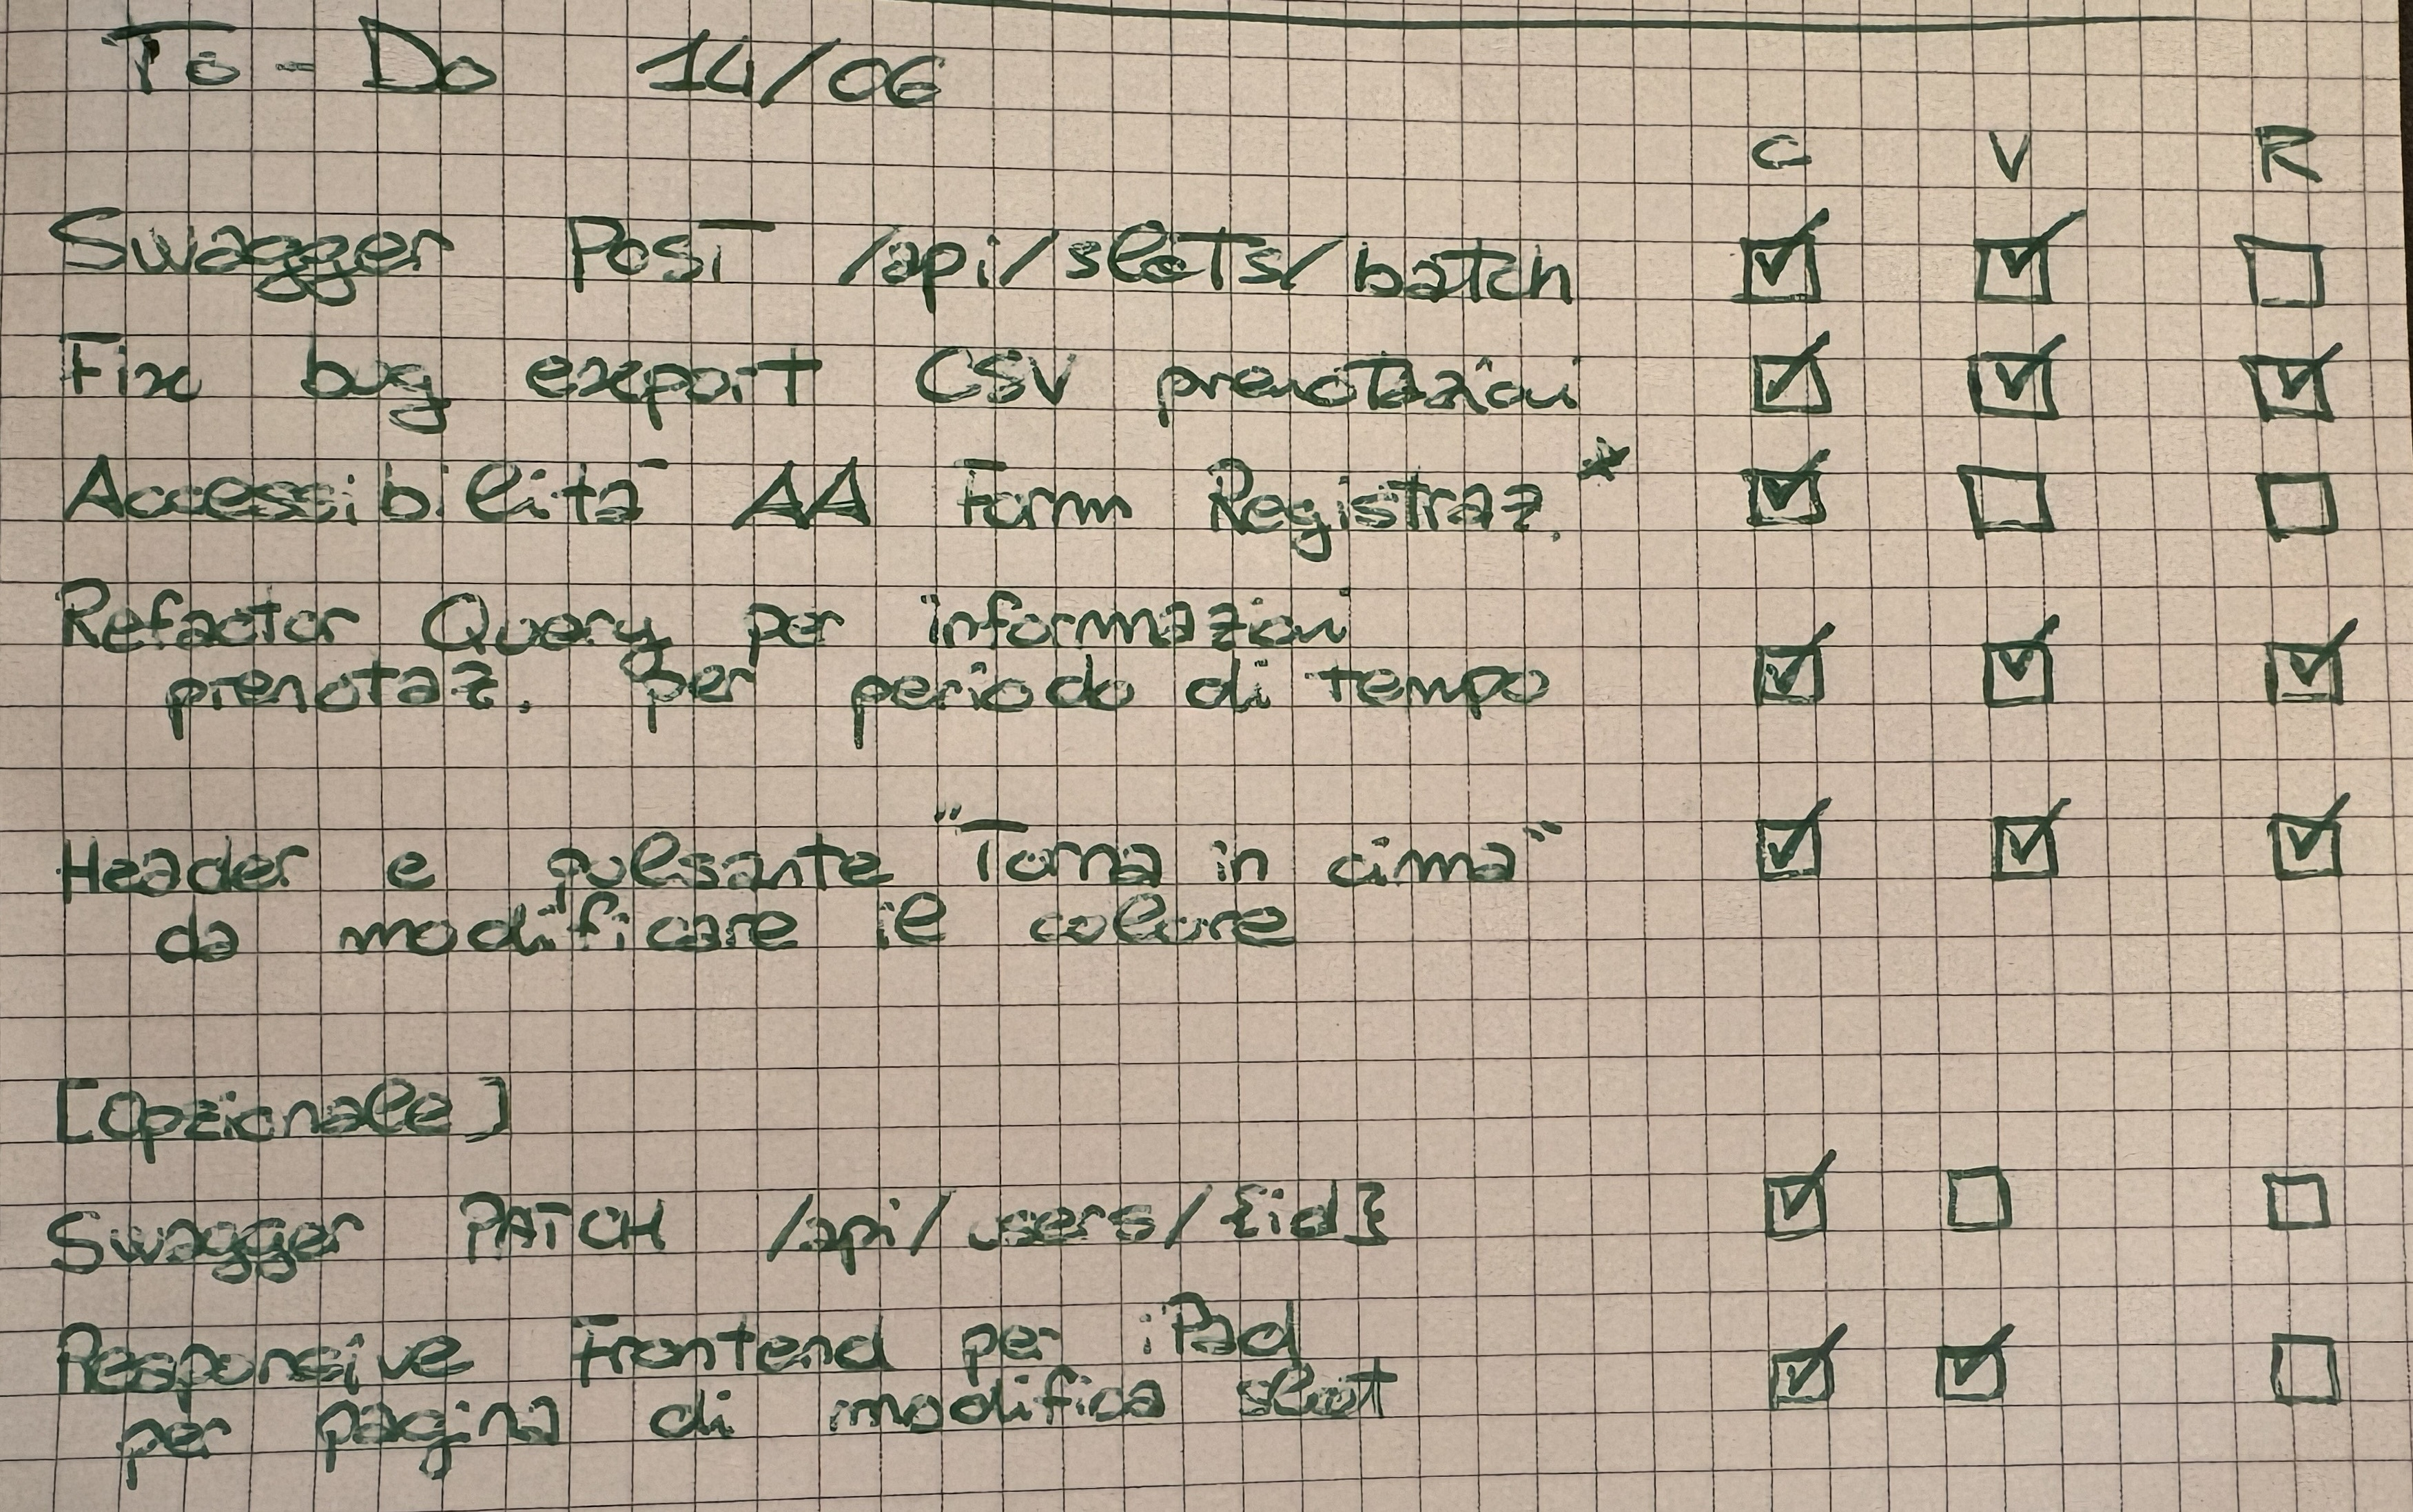
\includegraphics[width=0.7\textwidth]{img/notes.jpg}
    \caption{Appunti cartacei relativi alla fase di analisi del dominio applicativo e modellazione preliminare.}
    \vspace{0.1cm}
    {\footnotesize Elaborazione originale dell'autore\par}
    \label{fig:appunti_analisi}
\end{figure}

\begin{figure}[H]
    \centering
    \includegraphics[width=0.7\textwidth]{img/analysis.png}
    \caption{Sistema di tracciamento giornaliero basato su criteri di completamento, verifica e revisione.}
    \vspace{0.1cm}
    {\footnotesize Elaborazione originale dell'autore\par}
    \label{fig:todo_list}
\end{figure}

La natura esplorativa del progetto ha richiesto inoltre una costante attività di auto-formazione. Ho supportato ogni fase di implementazione mediante la consultazione sistematica delle documentazioni ufficiali delle tecnologie adottate: la guida di riferimento di React \cite{react_docs}, il portale di Microsoft Learn per l'ecosistema .NET \cite{dotnet_docs} e la documentazione tecnica di Informix \cite{informix_docs}. Tale pratica non ha rappresentato un mero supporto all'implementazione, ma un'attività di analisi tecnica strutturata per comprendere le \textit{best practice} di ogni \textit{framework} e applicarle correttamente nel contesto aziendale.

\section{Il ciclo di vita e le sfide progettuali}
\label{sec:ciclo_vita_kargo}

Di seguito dettaglio come ho trasformato le specifiche iniziali in un applicativo funzionante, seguendo la sequenza analisi, progettazione, programmazione e verifica, e motivando le principali decisioni tecniche adottate.

\subsection{Analisi dei requisiti e validazione del prototipo}
\label{subsec:analisi_validazione}

Prima di avviare lo sviluppo vero e proprio, il tutor mi ha formalizzato i vincoli architetturali discussi nel capitolo precedente, introducendomi al progetto con il suo nome provvisorio: "\textit{Web Service} Prenotazione Scarichi". L'obiettivo primario consisteva nel fornire ai corrieri una piattaforma per registrarsi e prenotare le baie dei depositi, centralizzando il controllo delle richieste.

Sfruttando l'assenza di linee guida aziendali rigide per la stesura della documentazione preliminare, ho applicato i principi appresi nel corso di Ingegneria del \textit{Software} per condurre un'analisi dei requisiti strutturata. Ho adottato un approccio gerarchico: sono partito dalla definizione degli attori di sistema, per poi isolare le macro-operazioni e descrivere infine il flusso operativo sequenziale necessario all'utente per completare ogni azione. Questo metodo ha consentito di granulare i requisiti in maniera precisa, rendendoli direttamente implementabili e verificabili attraverso le \textit{checklist} giornaliere descritte nella Sezione~\ref{subsec:sviluppo_personale}.

Ho redatto un documento contenente questa descrizione del dominio, formulando i diagrammi dei casi d'uso tramite PlantUML --- uno strumento che genera diagrammi UML a partire da una sintassi testuale --- per tracciare visivamente ogni scenario di interazione. Successivamente, ho mappato i requisiti, consolidandoli all'interno di apposite tabelle di classificazione. La Figura~\ref{fig:diagramma_casi_uso} e la Figura~\ref{fig:requirements_table} mostrano un estratto del lavoro di analisi.

\begin{figure}[H]
    \centering
    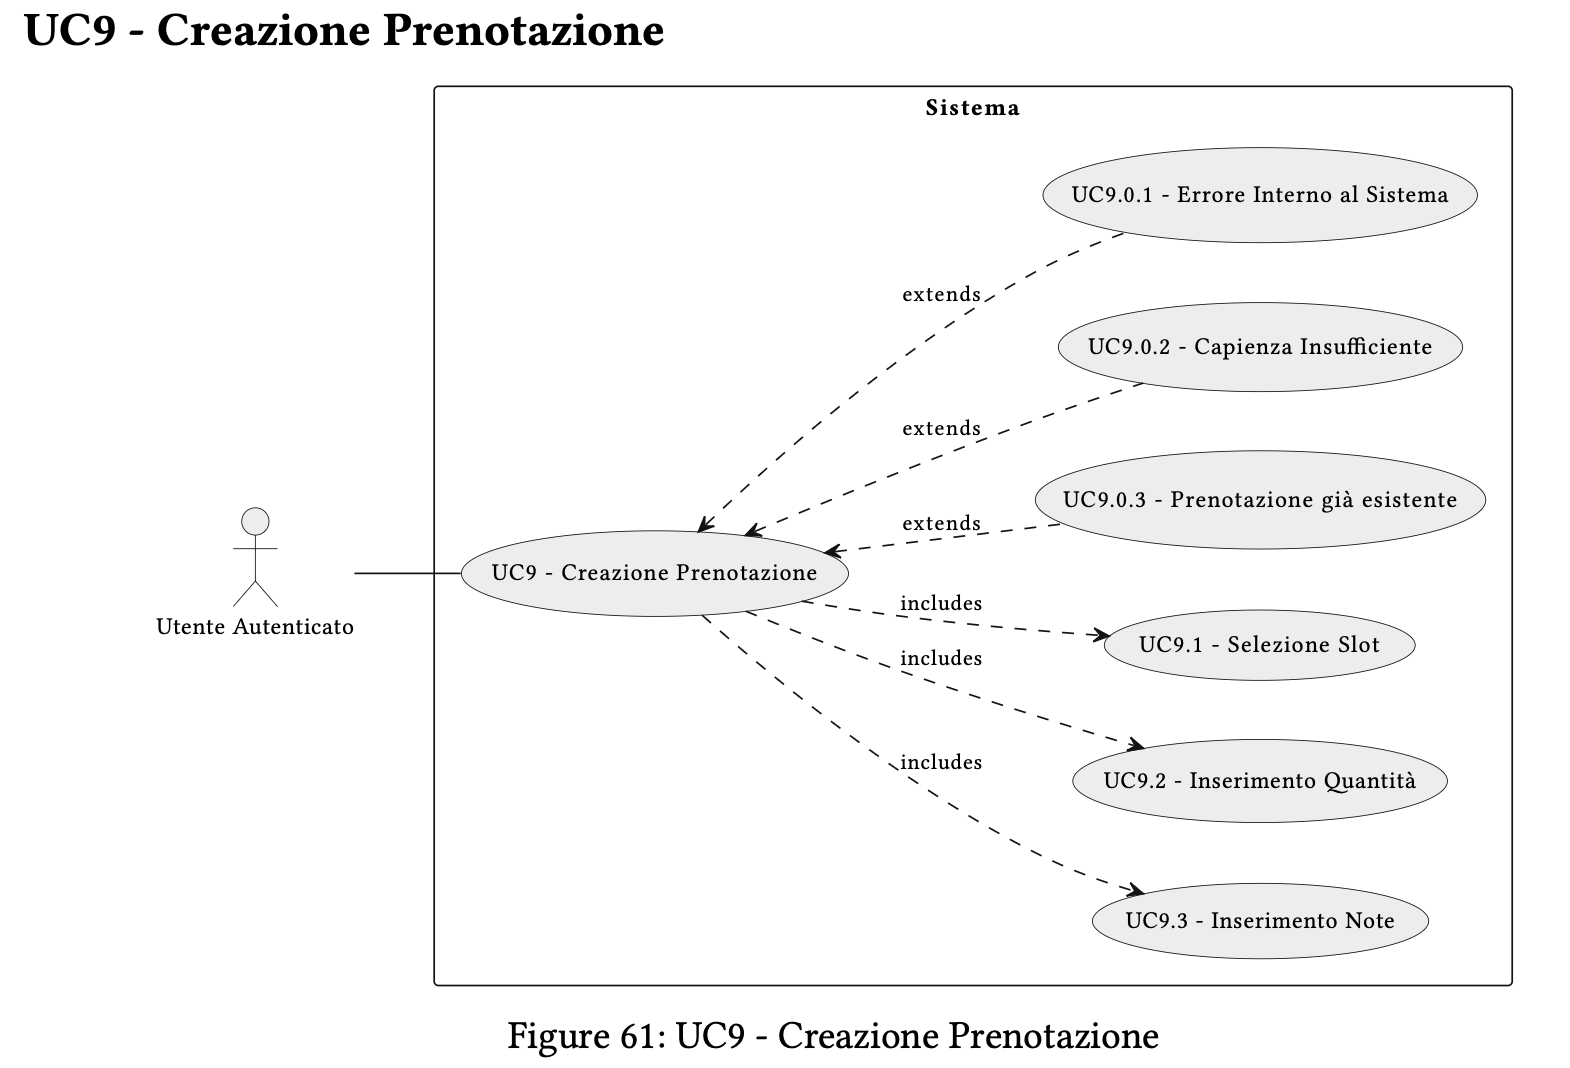
\includegraphics[width=0.7\textwidth]{img/uc.png}
    \caption{Estratto del diagramma dei casi d'uso generato tramite PlantUML.}
    \vspace{0.1cm}
    {\footnotesize Elaborazione originale dell'autore\par}
    \label{fig:diagramma_casi_uso}
\end{figure}

\begin{figure}[H]
    \centering
    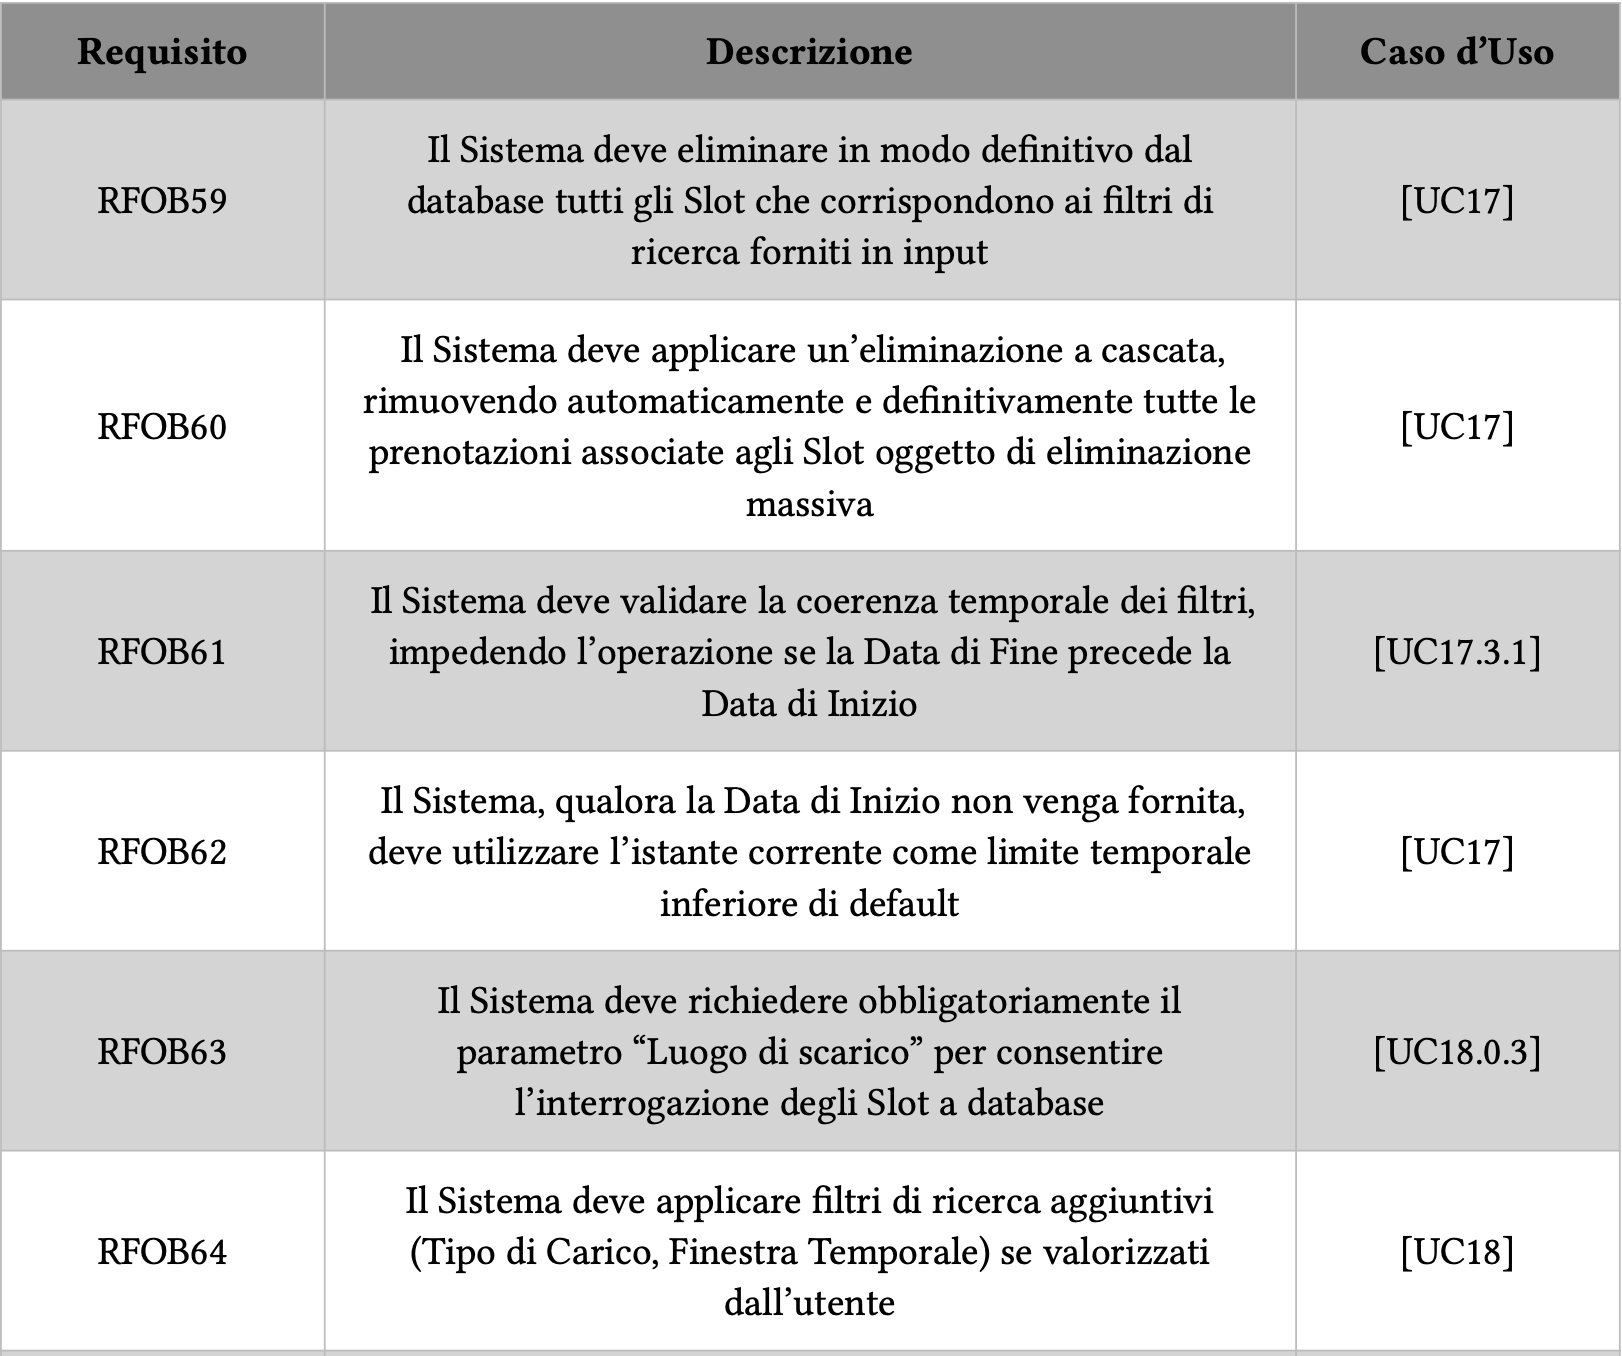
\includegraphics[width=0.8\textwidth]{img/requirements.png}
    \caption{Estratto della tabella di tracciamento dei requisiti funzionali.}
    \vspace{0.1cm}
    {\footnotesize Elaborazione originale dell'autore\par}
    \label{fig:requirements_table}
\end{figure}

Inizialmente, la mia propensione per la documentazione formale e la totale assenza di conoscenze pregresse sui linguaggi C\# e React hanno suscitato alcune perplessità nel tutor aziendale. Tuttavia, esaminando la precisione dei documenti prodotti, egli ha compreso il valore del rigore analitico e mi ha incitato a proseguire con questa metodologia.

Forte dei requisiti validati, ho sviluppato in circa tre settimane un primo prototipo funzionante, con lo scopo di acquisire dimestichezza con lo \textit{stack} tecnologico. Durante la stesura di questo eseguibile preliminare, ho ideato il nome definitivo dell'applicativo --- Kargo --- e ne ho disegnato il logo ufficiale, richiamando la veste cromatica dell'azienda committente, come illustrato in Figura~\ref{fig:logo_kargo}.

\begin{figure}[H]
    \centering
    
\includegraphics[width=0.4\textwidth]{img/KargoLogo.png}
    \caption{Logo dell'applicativo Kargo.}
    \vspace{0.1cm}
    {\footnotesize Elaborazione originale dell'autore\par}
    \label{fig:logo_kargo}
\end{figure}

\subsection{Evoluzione del dominio applicativo e sicurezza}
\label{subsec:evoluzione_dominio}

La rapidità con cui ho consegnato il prototipo ha fornito alla dirigenza tecnica l'opportunità di espandere il raggio d'azione di Kargo. Il tutor ha spostato l'attenzione dal semplice utilizzatore finale alla figura dell'amministratore, con l'intento di rendere il sistema autosufficiente e capace di autogestirsi integralmente.

Ho implementato funzionalità che garantiscono agli amministratori il controllo completo sulle prenotazioni e sugli intervalli temporali, operando sia su singole istanze sia tramite elaborazioni massive (\textit{batch}). Per potenziare il supporto decisionale, ho integrato procedure di esportazione dei dati in formato PDF e CSV, consentendo agli amministratori di estrarre \textit{report} dettagliati delle prenotazioni associate a ogni specifico \textit{slot}. Inoltre, per agevolare l'auto-formazione degli utenti, ho introdotto un modulo di consultazione documentale che espone dinamicamente il manuale utente o il manuale amministratore in base al profilo di autorizzazione del soggetto autenticato.

Parallelamente, ho rilevato la necessità di innalzare gli standard di sicurezza. Ho integrato un sistema di validazione visiva (\textit{captcha}) per scongiurare registrazioni automatizzate da parte di \textit{bot}. Inoltre, il tutor ha imposto un meccanismo di attivazione degli account tramite \gls{otp} --- ovvero un codice numerico monouso --- per prevenire furti d'identità aziendale. 

Per la gestione delle sessioni, ho contestato l'approccio iniziale che prevedeva il passaggio di dati sensibili in chiaro tramite richieste HTTP GET, proponendo e implementando in sua sostituzione l'adozione di \gls{jwt} --- token crittografici compatti impiegati per il trasferimento sicuro di asserzioni tra le parti --- strutturati in \textit{Access} e \textit{Refresh Token} e archiviati in \textit{cookie} \textit{HttpOnly}, inaccessibili agli \textit{script} lato \textit{client}.

\subsection{Progettazione architetturale e direttive di codifica}
\label{subsec:architettura_codifica}

L'evoluzione dei requisiti ha progressivamente concentrato la complessità del sistema nelle regole di dominio, rendendo inefficace un approccio procedurale classico. Ho pertanto adottato il modello di sviluppo guidato dal dominio (\gls{ddd}), necessario per governare vincoli stringenti: le prenotazioni dovevano rispettare un tempo limite di registrazione; il sistema doveva condizionare dinamicamente le operazioni permesse in base allo stato dell'utente; la generazione \textit{batch} richiedeva controlli incrociati per impedire sovrapposizioni e rispettare il limite massimo di porte disponibili.

Per proteggere questa logica di \textit{business}, ho adottato l'architettura esagonale (\textit{Ports and Adapters}): l'utilizzo di interfacce, ovvero le porte, ha delegato a specifici \textit{adapter} la responsabilità di dialogare con la base dati corretta, rendendo il sistema agnostico rispetto alle differenze strutturali tra il \textit{database} di collaudo e quello di produzione. Tramite PlantUML ho strutturato i diagrammi delle classi partendo dal \textit{Domain Layer}, fino ai \textit{Controller} (Figura~\ref{fig:diagramma_classi}).

\begin{figure}[H]
    \centering
    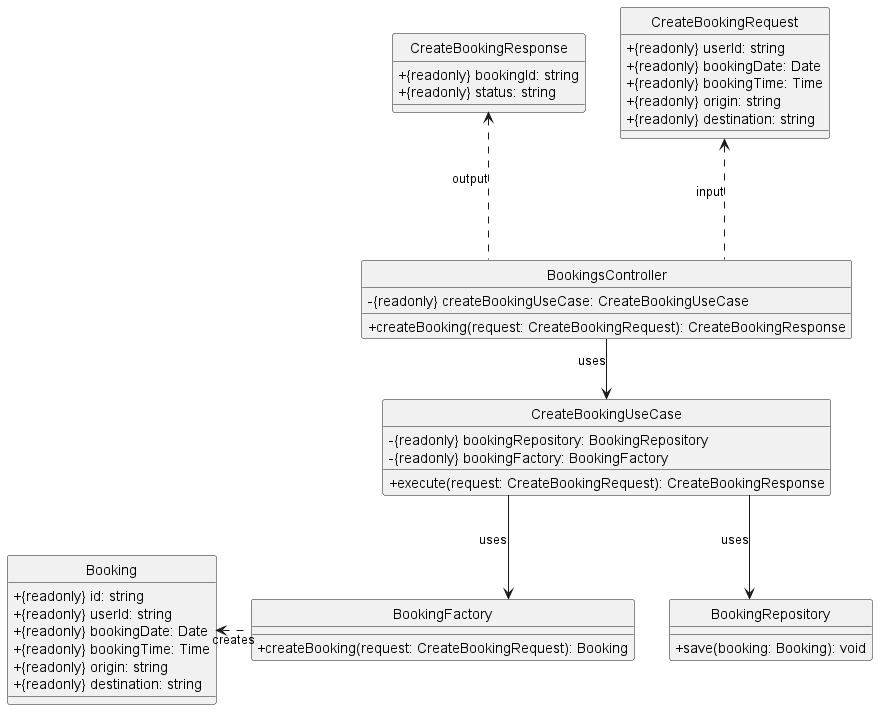
\includegraphics[width=0.8\textwidth]{img/design.jpeg}
    \caption{Modellazione delle classi di dominio e del livello applicativo.}
    \vspace{0.1cm}
    {\footnotesize Elaborazione originale dell'autore\par}
    \label{fig:diagramma_classi}
\end{figure}

Nella stesura del codice, ho applicato i principi \gls{solid} per la creazione di \textit{software} manutenibile e disaccoppiato:
\begin{itemize}
    \item \textbf{Inversione del controllo e iniezione delle dipendenze:} ho svincolato le classi dalla loro implementazione concreta mediante interfacce astratte, garantendo modularità e intercambiabilità.
    \item \textbf{Responsabilità singola:} ogni entità assolve esclusivamente a un singolo compito logico.
    \item \textbf{Segregazione e Sostituzione di Liskov:} il codice di dominio interagisce con interfacce minimali, delegando agli \textit{adapter} la traduzione dei contratti astratti.
\end{itemize}

Sul livello \textit{frontend} in React e TypeScript, ho configurato un ambiente di analisi statica (\textit{linting}) tramite ESLint e Prettier. Infine, per preservare le prestazioni, ho implementato un gestore universale delle eccezioni --- evitando la duplicazione di costrutti \texttt{try-catch} in violazione del principio \gls{dry} --- e un \textit{rate limiter} sulle \gls{api} per proteggere le operazioni critiche.

A titolo esemplificativo, la Figura~\ref{fig:create_booking_usecase} riporta l'implementazione del caso d'uso primario per la generazione delle prenotazioni. Il frammento evidenzia l'applicazione pratica dell'Iniezione delle Dipendenze --- le interfacce di accesso ai dati vengono passate al costruttore --- e l'incapsulamento delle regole di \textit{business}. Il sistema delega la persistenza agli \textit{adapter} infrastrutturali tramite il \textit{pattern Unit of Work} esclusivamente dopo aver validato rigorosamente i vincoli di dominio (quali lo stato dell'utente, la capienza dello \textit{slot} e le tempistiche di scarico).

\begin{figure}[H]
    \centering
    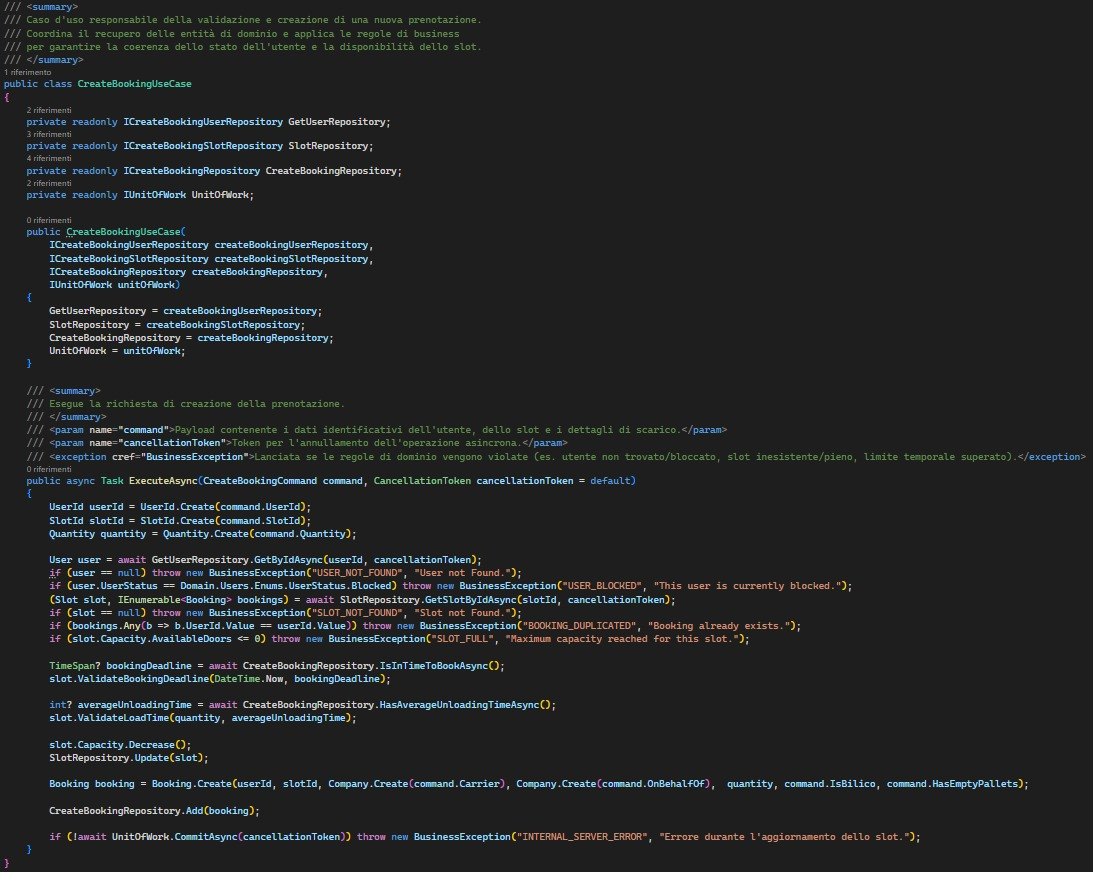
\includegraphics[width=1.0\textwidth]{img/code.jpeg}
    \caption{Implementazione del caso d'uso di creazione prenotazione.}
    \vspace{0.1cm}
    {\footnotesize Elaborazione originale dell'autore\par}
    \label{fig:create_booking_usecase}
\end{figure}

\subsection{Verifica e validazione delle funzionalità}
\label{subsec:verifica_validazione}

Ho interpretato la fase di verifica come un elemento strutturale continuo del ciclo di sviluppo. Ho condotto la validazione dei requisiti in modo strettamente incrementale, sottoponendo ogni funzionalità implementata a riscontri operativi diretti per garantirne la piena conformità.

Per collaudare il \textit{backend}, mi sono avvalso principalmente di Postman per simulare i percorsi tracciati nei diagrammi dei casi d'uso e di Swagger per documentare e testare attivamente gli \textit{endpoint} esposti. Sul versante \textit{frontend}, ho validato l'applicativo tramite esecuzioni dirette nell'ambiente di sviluppo locale, focalizzandomi sull'accessibilità visiva e comportamentale con il supporto dei DevTools di Google Chrome. Ho verificato la reattività (\textit{responsiveness}) dell'applicativo su schermi \textit{desktop}, \textit{tablet} e terminali mobili. 

Sebbene abbia strutturato l'ambiente TypeScript per supportare la scrittura di \textit{unit test} al fine di garantire una solida base per future integrazioni, la validazione del presente prototipo si è basata su un collaudo empirico iterativo, integrato dalle revisioni periodiche condivise con il tutor aziendale per stabilire l'approvazione funzionale dei moduli.

\section{Risultati qualitativi e quantitativi}
\label{sec:risultati_kargo}

Al termine delle ore previste per la stesura del codice, ho sottoposto l'applicativo Kargo alla valutazione finale della dirigenza tecnica. L'esito del progetto si articola su due dimensioni d'analisi: la percezione del prodotto dal lato utente e la misurazione delle metriche ingegneristiche di copertura.

\subsection{Il prodotto dal lato utente}
\label{subsec:risultati_qualitativi}

Sul piano qualitativo, Kargo si presenta come un applicativo reattivo, solido e fortemente orientato all'usabilità. Sebbene abbia sviluppato l'applicativo per l'uso interno logistico --- un settore che spesso subordina l'estetica alla pura funzionalità --- ho dedicato particolare attenzione all'interfaccia utente, garantendo il rispetto degli standard di accessibilità \textit{Web Content Accessibility Guidelines} (WCAG) di livello AA e, in alcuni componenti critici, di livello AAA. Ho verificato tale conformità analizzando i rapporti di contrasto cromatico, implementando la navigazione completa tramite tastiera e utilizzando i \textit{tag} semantici HTML5 controllati mediante gli strumenti di ispezione del \textit{browser}.

L'interfaccia guida gli attori del sistema attraverso flussi operativi chiari. Per gestire la notevole mole di dati derivante dall'espansione del dominio, ho progettato e implementato funzioni avanzate di ricerca e filtraggio dinamico. Sia i corrieri, nella consultazione degli \textit{slot} liberi, sia gli amministratori, nel monitoraggio globale del deposito, possono interrogare la base dati in tempo reale, isolando le prenotazioni per data, stato o tipologia di carico con risposte visive immediate. 

Le Figure dalla~\ref{fig:kargo_selezione_slot} alla~\ref{fig:kargo_modifica_slot} dimostrano la resa finale dell'applicativo, evidenziando la funzionalità di creazione della prenotazione lato corriere e di gestione delle prenotazioni lato amministratore.

\begin{figure}[H]
    \centering
    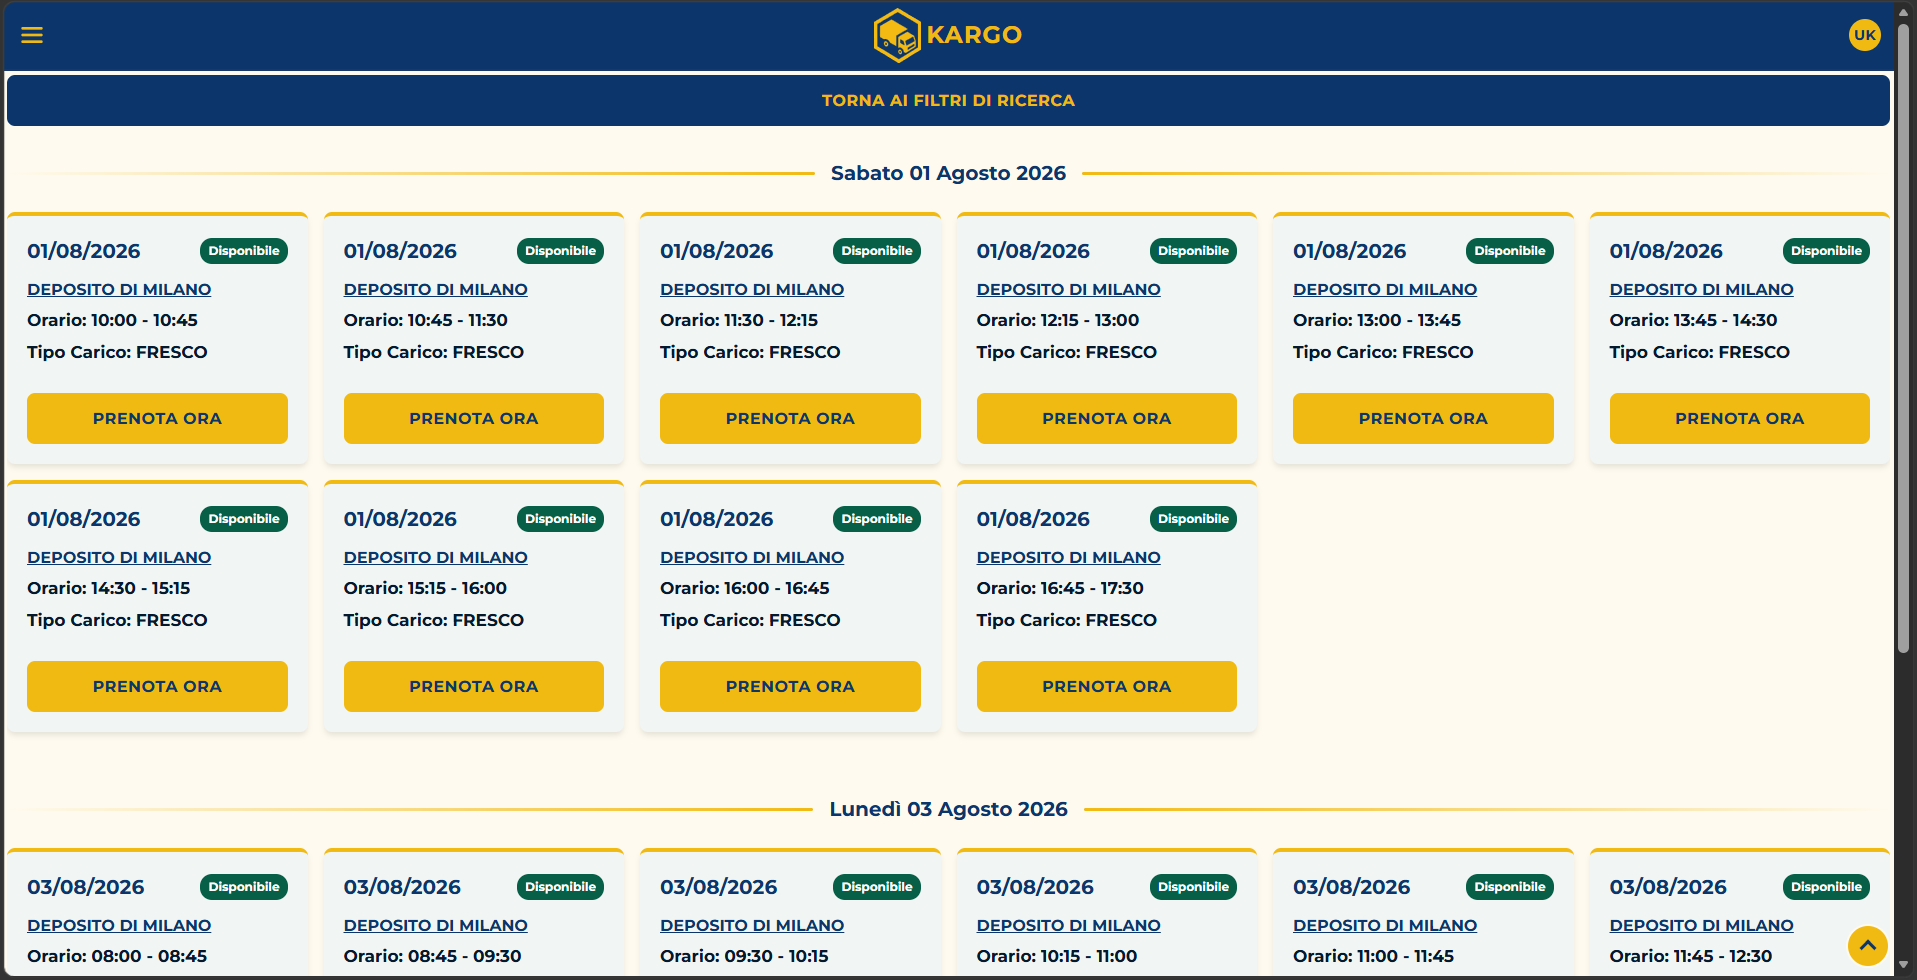
\includegraphics[width=1.0\textwidth]{img/viewSlotsForBookingPage2.png} 
    \caption{Interfaccia di selezione della finestra temporale di prenotazione.}
    \vspace{0.1cm}
    {\footnotesize Elaborazione originale dell'autore\par}
    \label{fig:kargo_selezione_slot}
\end{figure}

\begin{figure}[H]
    \centering
    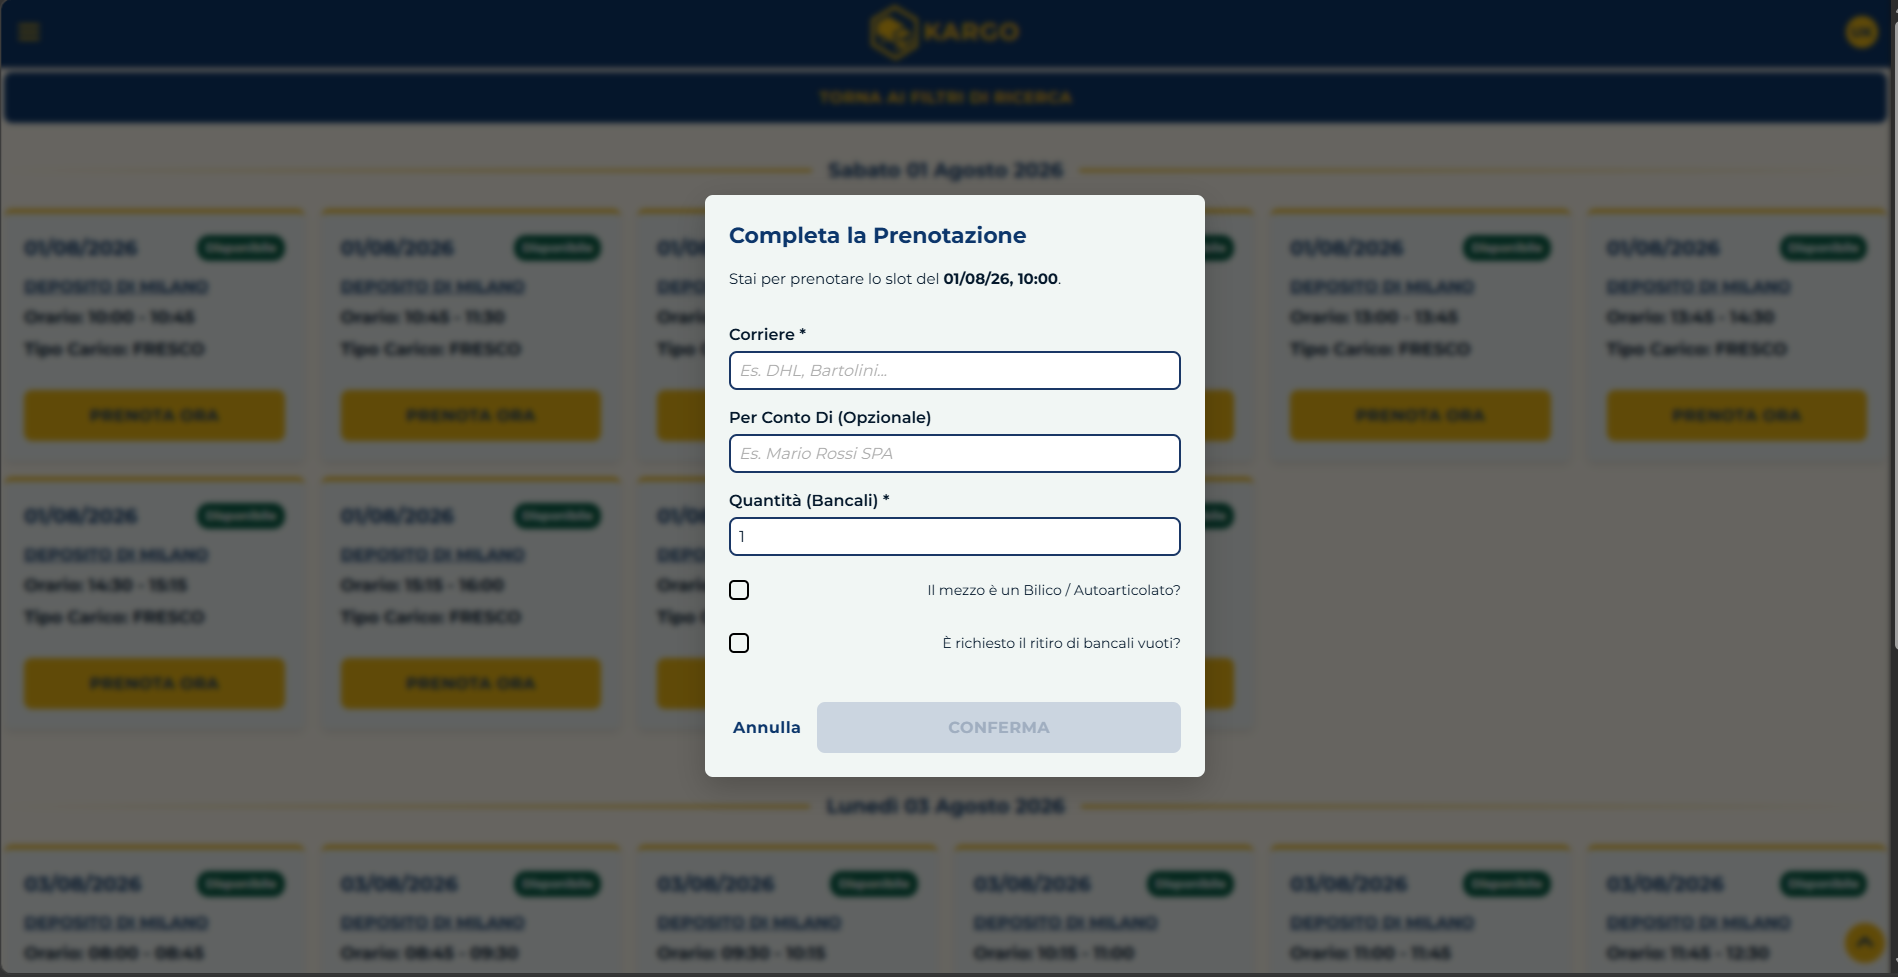
\includegraphics[width=0.9\textwidth]{img/completeBooking.png} 
    \caption{Dettaglio sul completamento della prenotazione.}
    \vspace{0.1cm}
    {\footnotesize Elaborazione originale dell'autore\par}
    \label{fig:kargo_completamento_prenotazione}
\end{figure}

\begin{figure}[H]
    \centering
    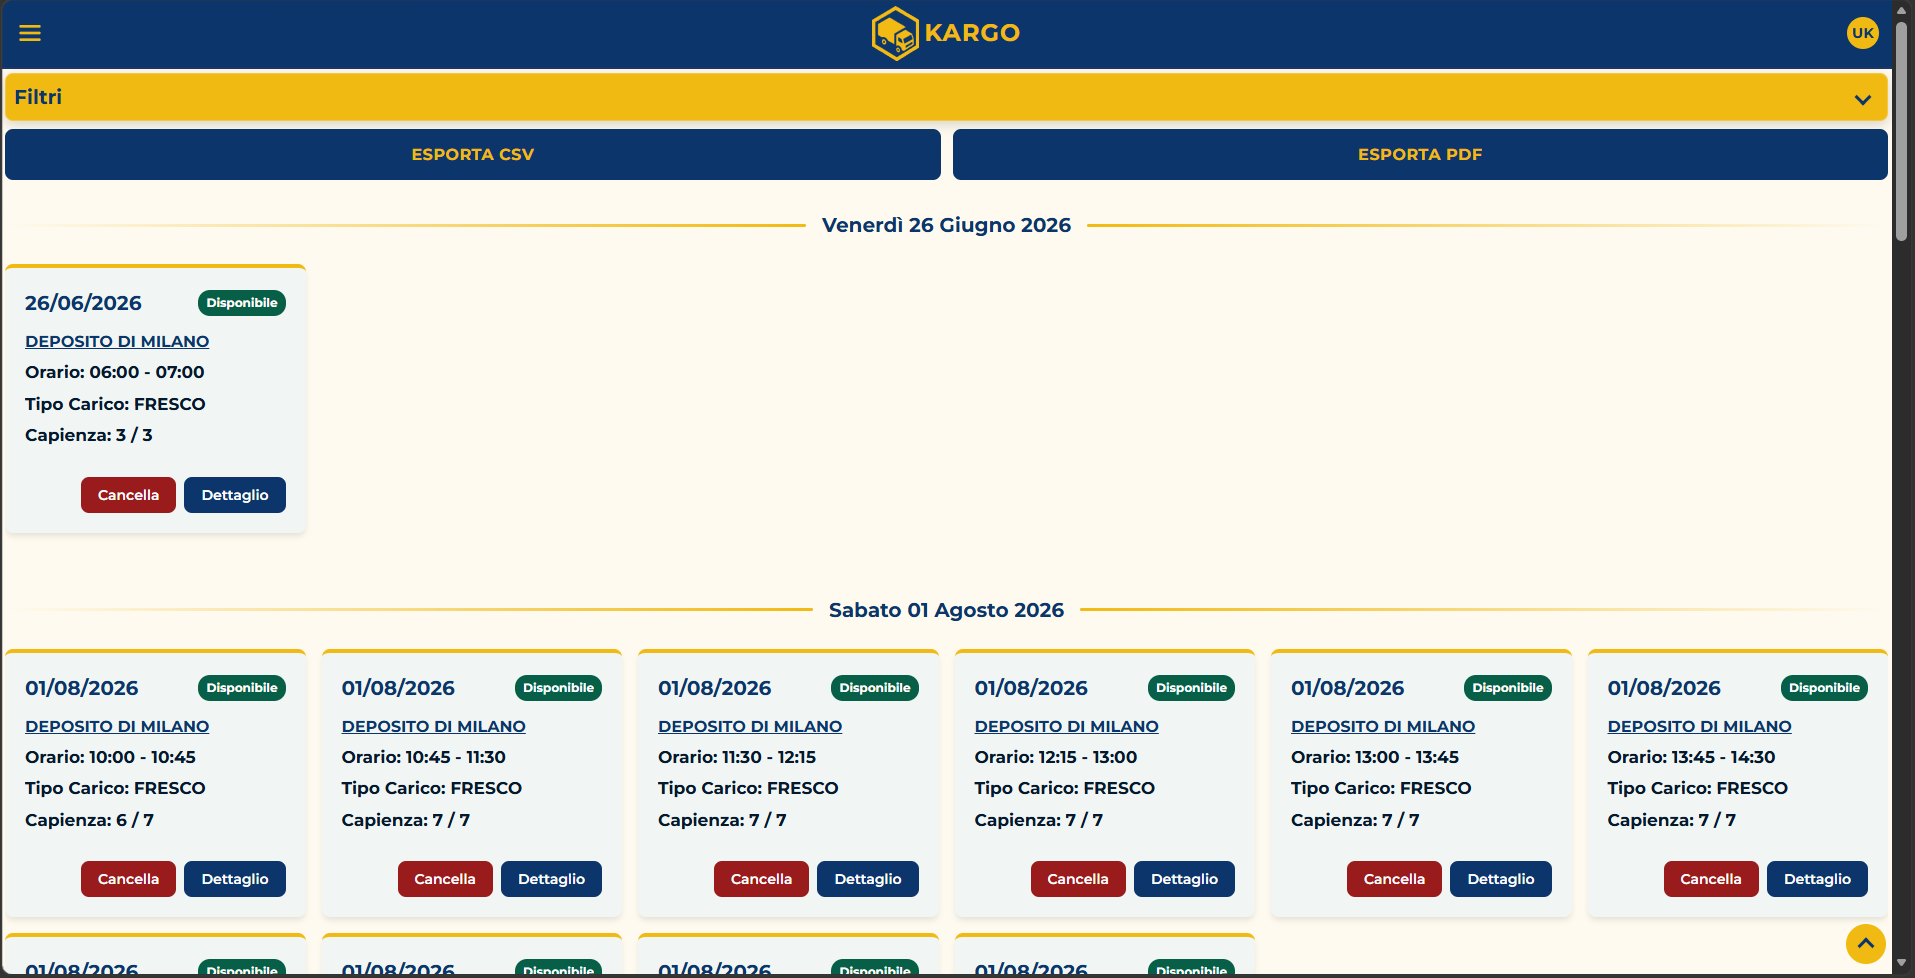
\includegraphics[width=0.9\textwidth]{img/viewSlotsPage2.png} 
    \caption{Visualizzazione della gestione degli slot temporali.}
    \vspace{0.1cm}
    {\footnotesize Elaborazione originale dell'autore\par}
    \label{fig:kargo_gestione_slot}
\end{figure}

\begin{figure}[H]
    \centering
    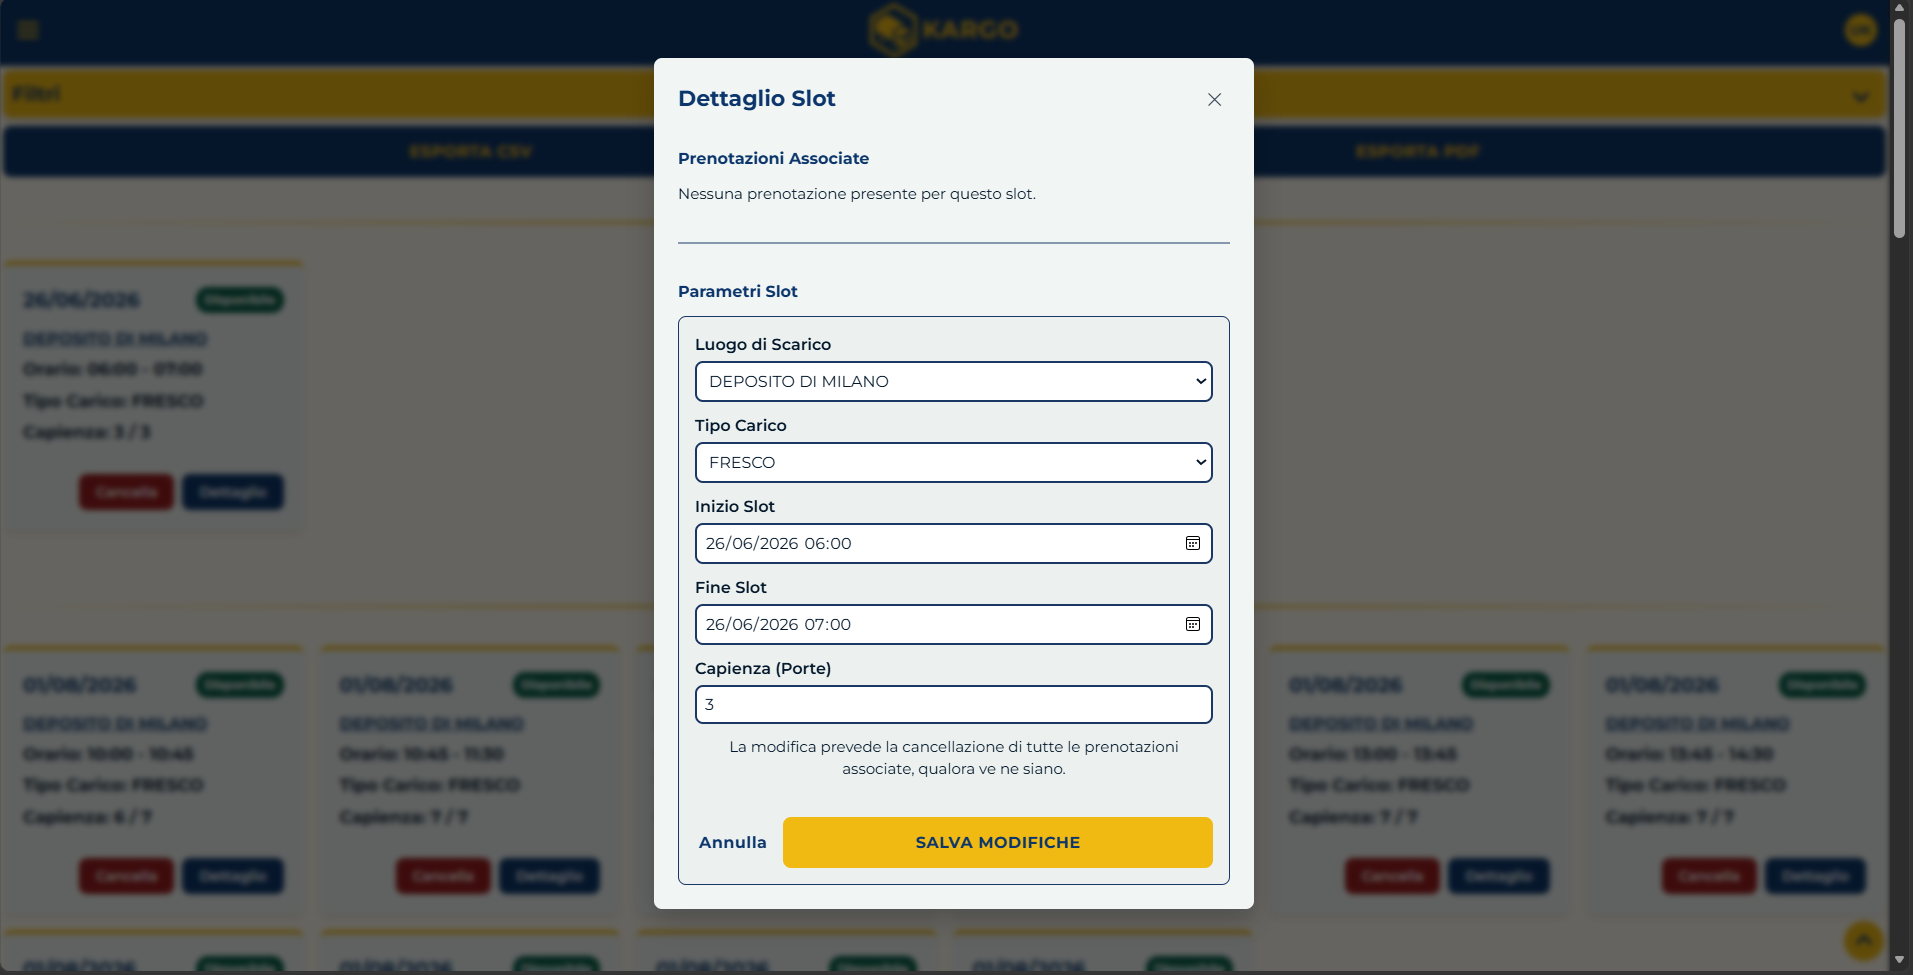
\includegraphics[width=0.9\textwidth]{img/modifySlot.png} 
    \caption{Dettaglio sulla gestione degli slot temporali.}
    \vspace{0.1cm}
    {\footnotesize Elaborazione originale dell'autore\par}
    \label{fig:kargo_modifica_slot}
\end{figure}

\subsection{Copertura e metriche di progetto}
\label{subsec:risultati_quantitativi}

Sotto il profilo quantitativo, i risultati testimoniano il pieno conseguimento degli obiettivi aziendali e l'efficacia strategica dello \textit{stage} delineati nel Capitolo~\ref{chap:strategia}. Nonostante il tutor abbia richiesto un massiccio ampliamento del dominio a lavori già avviati, ho consegnato la \textit{release} definitiva dell'applicativo con circa una settimana di anticipo rispetto alle scadenze originarie concordate con l'azienda.

Dal punto di vista della copertura funzionale, ho mappato e soddisfatto integralmente le richieste del committente. La Tabella~\ref{tab:riepilogo_requisiti} illustra il riepilogo quantitativo dei requisiti individuati in fase di analisi, suddivisi per tipologia e grado di adempimento.

\begin{table}[H]
    \centering
    \begin{tabular}{p{0.3\textwidth} c c c}
        \hline
        \textbf{Tipologia Requisito} & \textbf{Obbligatori} & \textbf{Desiderabili} & \textbf{Opzionali} \\
        \hline
        Requisiti Utente & 24 & 1 & 1 \\
        Requisiti Funzionali & 80 & 1 & 0 \\
        Requisiti non Funzionali & 3 & 1 & 2 \\
        Requisiti di Interfaccia & 35 & 3 & 1 \\
        \hline
        \textbf{Totale} & \textbf{142} & \textbf{6} & \textbf{4} \\
        \hline
    \end{tabular}
    \caption{Riepilogo quantitativo della tracciabilità dei requisiti di progetto.}
    \vspace{0.1cm}
    {\footnotesize Valori assoluti derivati dalla matrice di tracciamento dei requisiti validata dal tutor aziendale.\par}
    \label{tab:riepilogo_requisiti}
\end{table}

A livello di volumetria del prodotto, il \textit{repository} finale si compone di una ricca infrastruttura logica, quantificabile in circa 20 \textit{endpoint} \gls{api} esposti lato \textit{backend}, supportati da svariate decine di classi di dominio in C\# e molteplici componenti \textit{custom} in React sviluppati \textit{ex novo}. A questa produzione informatica ho affiancato il parallelo lavoro di stesura documentale, concretizzatosi nella redazione formale del documento di analisi dei requisiti iniziale e nella produzione di due guide operative complete: il manuale utente, destinato ai corrieri, e il manuale amministratore, riservato al personale della logistica interna.

Infine, coerentemente con le direttive operative interne descritte nella Sezione~\ref{subsec:verifica_validazione}, non ho prodotto metriche automatizzate di \textit{code-coverage}. Sebbene abbia configurato l'ambiente per supportare rigide analisi statiche mediante ESLint, ho basato la validazione finale sull'esito positivo dei rigorosi collaudi empirici e visivi condotti congiuntamente al \textit{team} tecnico di Ergon Informatica, decretando il successo complessivo dello \textit{stage}.
    \chapter{Valutazione retrospettiva}
\label{chap:conclusioni}

\textit{Il presente capitolo propone una valutazione critica del percorso di tirocinio svolto. Attraverso l'analisi dei risultati conseguiti rispetto agli obiettivi prefissati e una riflessione sulla maturazione professionale acquisita, si intende fornire una sintesi del valore dell'esperienza in Ergon Informatica. Il capitolo si conclude con una disamina sul rapporto tra il bagaglio formativo universitario e le competenze richieste dal mondo del lavoro, tracciando un bilancio finale sul percorso accademico intrapreso.}

\section{Analisi dei risultati e maturazione professionale}
Questa sezione valuta, su base oggettiva, il grado di soddisfacimento degli obiettivi prefissati in sede di pianificazione. Si analizzano le performance ottenute confrontandole con le aspettative aziendali, evidenziando come la gestione autonoma di un progetto \textit{enterprise} — unita alla necessità di apprendere rapidamente \textit{framework} e tecnologie inedite — abbia favorito una crescita professionale significativa. L'attenzione si focalizza sulla capacità di allineare il proprio operato agli standard e alla visione dell'azienda, superando la prospettiva puramente individuale in favore di una soluzione tecnica coerente con le necessità produttive e di mercato.

\section{Bilancio formativo: dall'università al mondo del lavoro}
Viene analizzato il divario tra le competenze acquisite durante il corso di studi e quelle richieste per l'operatività quotidiana. Si discute come l'approccio ingegneristico fornito dall'Università di Padova abbia costituito la base metodologica necessaria per affrontare il tirocinio, identificando al contempo le aree di competenza che hanno richiesto un maggior adattamento. Il capitolo si chiude con una riflessione retrospettiva sul percorso accademico, riconoscendo il ruolo dei singoli insegnamenti nel fornire gli strumenti teorici necessari a comprendere, a posteriori, l'importanza della rigorosità scientifica e della pianificazione nel contesto professionale.

\newpage

    \pagenumbering{roman}
    \backmatter
    \printglossary[type=\acronymtype, title=Acronimi e abbreviazioni, toctitle=Acronimi e abbreviazioni]
    \printglossary[type=main, title=Glossario, toctitle=Glossario]
    %\input{references/bibliography}
    %\input{references/webliography}
\end{document}